\documentclass{article}

%packages
\usepackage{geometry}
\usepackage{polski}
\usepackage[utf8]{inputenc}
\usepackage{hyperref}
\usepackage{graphicx}
\graphicspath{{./assets/}}

% Margin options
\geometry{top=2.5cm}
\geometry{bottom=2.5cm}
\geometry{left=2.5cm}
\geometry{right=2.5cm}

% title
\title{Tworzenie Aplikacji na iOS}
\author{Witold Bobrowski\\Uniwersytet Jagielloński w Krakowie}
\date{Wrzesień 2018}

% Document
\begin{document}

% Title
\maketitle

%
% Section: Introduction
%
\section*{Wstęp}
W tym artykule postaram się przybliżyć proces tworzenia aplikacji
mobilnych na system operacyjny Apple iOS\@. Opowiem o najpopularniejszych 
narzędziach, wytycznych Apple, dobrych praktykach, społeczności oraz 
zaprezentuję przykładową aplikację. Aplikacja posłuży mi za punkt odniesinia 
do tych konceptów oraz paradygmatów, które tutaj przedstawię. Kod źródłowy 
zostanie udostepniony wraz z tym dokumentem, a więc zachęcam do zapoznania się 
z zawartością.


%
% Section: Environment 
%
\section*{Środowisko}

\begin{figure}[h]
\centering
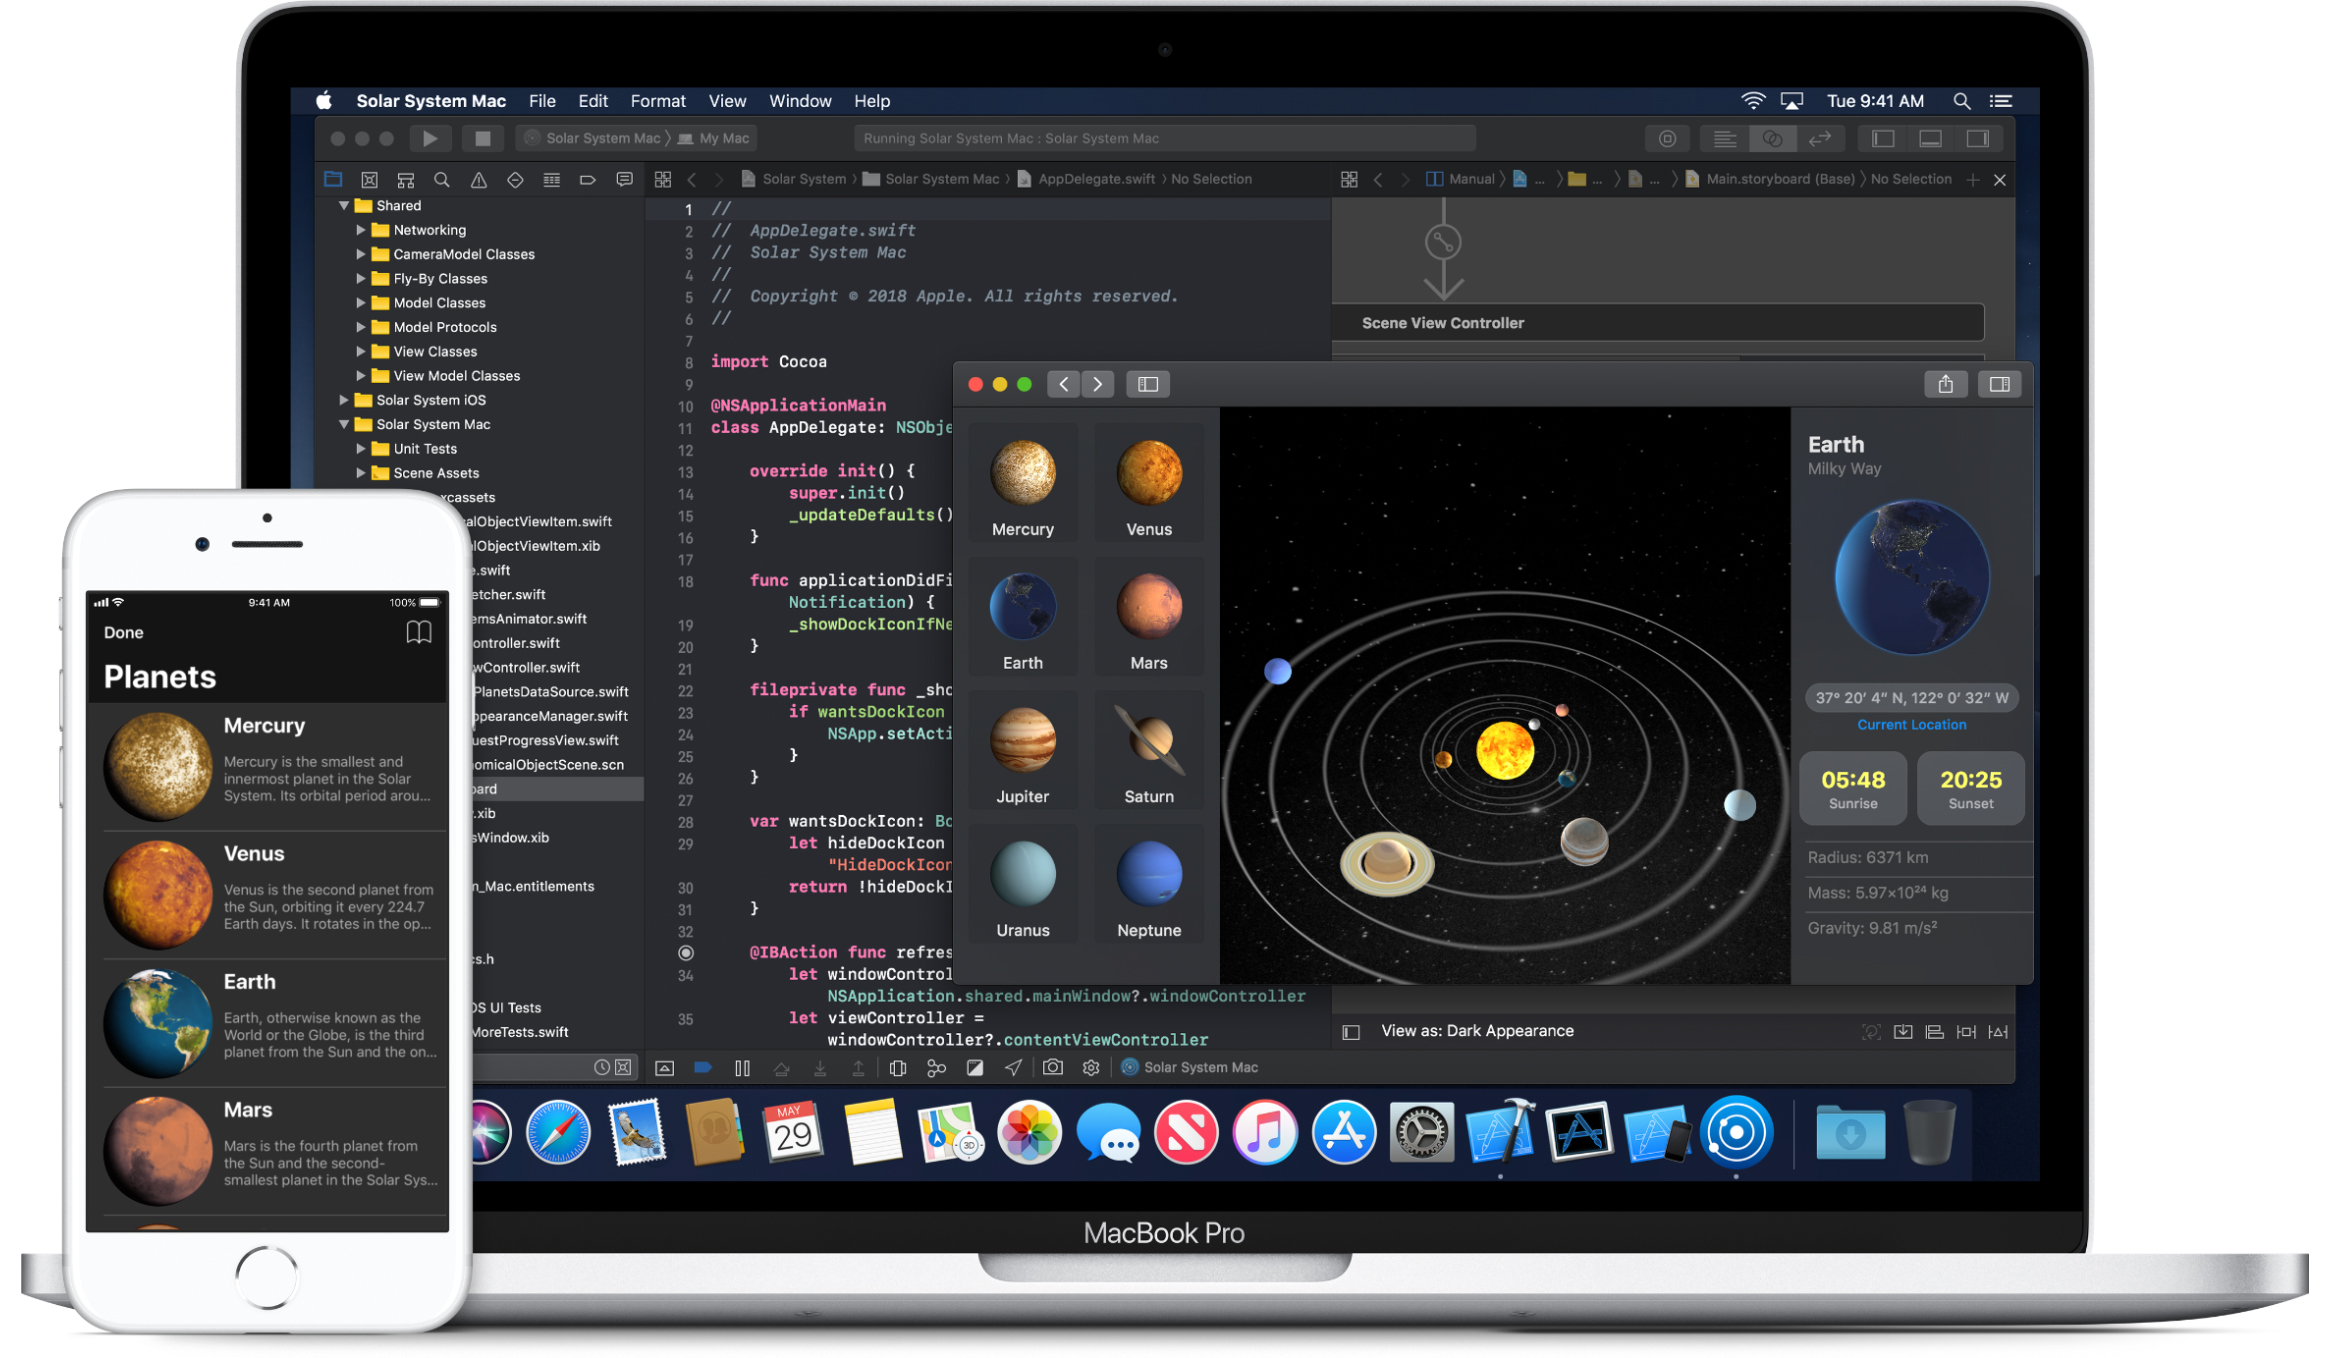
\includegraphics[width=12cm]{image-develop-hero-large_2x}
\caption{Źródło: \url{https://developer.apple.com/develop/}}
\end{figure}

\subsection*{macOS}
Na środowisko programisty tworzącego aplikaje na iOS, składa sie kilka elementów.
Przedewszystkim jest to system \textbf{macOS}, który jest dostępny jedynie na 
komputery produkowane przez Apple. Ten wymaganie powoduje, że wiele osób nie ma
nawet okazji zainteresować się tworzeniem appek na iOS bo najzwyczajniej w świecie
nie posiadają odpowiedniej maszyny. Macintosh nie cieszył się nigdy wielką
popularnością w polsce, a dla studenta może być poprostu nieosiągalny ze względu
na swoją cenę, która umiesza go w kategorii produktów premium. Technicznie jest
możliwe uruchomienie systemu na wirtualnej maszynie, bądź tak zwanym `Hackintoshu'
czyli PCecie, który dzięki zbliżonym komponentom do prawdziwego Maca pozwala przy
odrobinie wysiłku na instalację systemu macOS\@.

\subsection*{iPhone, iPad}
Naturalnie wydawało by się aby następnie wspomnieć o jakimś urządzenie z iOS, na
którym bedziemy uruchamiać aplikację. Na szczęście w naszym pakiecie narzędzi 
znajduje się symulator iOS, na którym bez problemu przetestujemy nasz kod.
Oczywiście fizyczne urządzenie pozwala nam na wiele więcej, dzięki niemu bedzięmy
mieli dostęp do wszystki funkcjonalności, których żaden symulator nie bedzie nam 
w stanie zapewnić. Więcej o symulatorze napiszę trochę później, przy okazji Xcode'a.
O ile ciężko wśród znajomych znaleźć kogoś z Macintoshem, o tyle łatwiej uda nam 
się wskazać kogoś z iPhonem. Telefony Apple na dobre wkroczyły na rynek polski i 
są coraz powszechniejsze. A to z pewnością dobra wiadomość dla programistów tworzących
oprogramowanie na tą platformę. Kolejnych urządzenie może być tablet z rodziny iPad
lub najmłodszy i zapewnie ostatni potomek reliktu przeszłości: iPod Touch. Każde
z tych urządzeń różni się od siebie, lecz co najważniejsze wszystkie posiadają 
jeden system operacyjny, który na każdym z nich identycznie. Warto jednak upewnić
się, że znajdujemy się wposiadaniu takiego urządzenia, które wspiera najnowszą
wersję iOS\footnote{Podczas pisania tego artykułu najnowszą wersją jest świeżo 
upieczony iOS 12, który wspiera tak stare urządzenia jak iPhone 5S z 2012 roku}.

\subsection*{Xcode}

\begin{figure}[h]
\centering
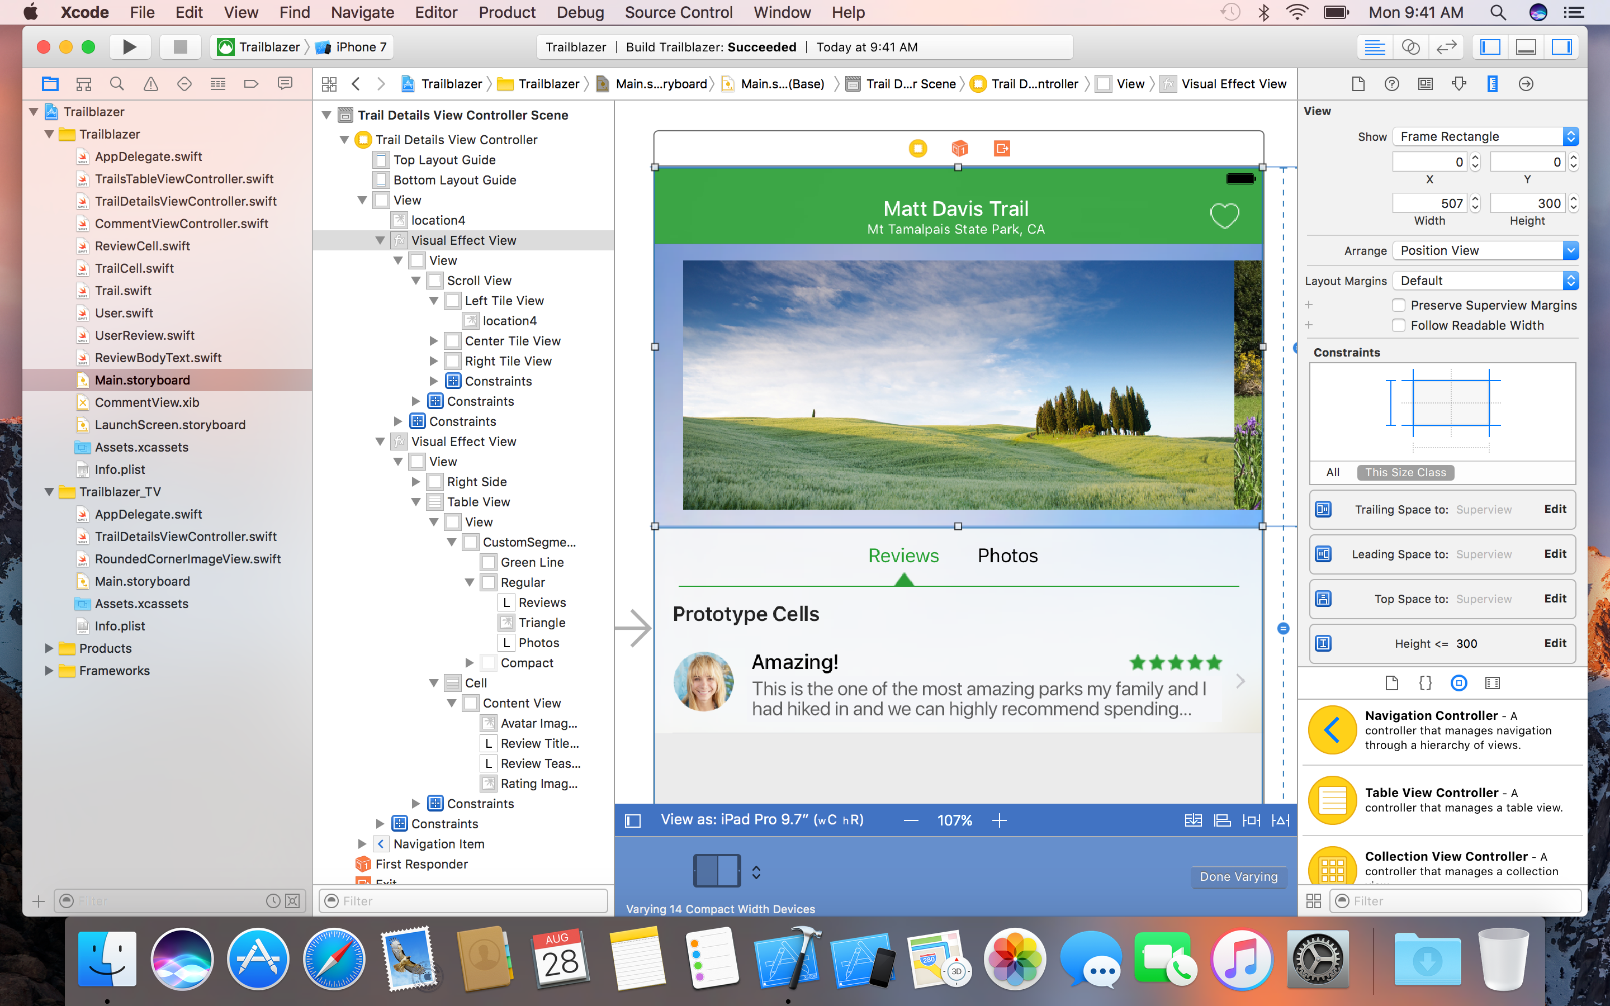
\includegraphics[width=12cm]{interface-builder_2x}
\caption{Źródło: \url{https://developer.apple.com/xcode/interface-builder/}}
\end{figure}

Wymagania hardware'owe mamy już za sobą, a więc przejdźmy do narzędzi jakimi będziemy
się posługiwać. Pierwszym z nich jest \textbf{Xcode}, który przedewszystkim pełni
rolę IDE, ale również posiada zestaw dodatkowych narzędzi, między innymi wcześniej
wspomniany \textbf{Simulator} czy \textbf{Instuments}, aplikacja posiadająca mnóstwo
narzędzi analizujących wynajność aplikacji działającej na urządzeniu bądź symulatorze.
Instuments to z pewnością narzędzie, z których każdy programista iOS musi się
zapoznać, a wskazane by było skożystać z niego przed wypuszczeniem swojej aplikacji
do AppStore.

Jeżeli chodzi o Xcode jako IDE to mamy do czynienia z dość zaawansowanym programem,
który udostępnia nam takie funkcjonalności jak \textbf{Interface Builder} czy
\textbf{View Debugger}. Jest całkiem spora szansa, że już obiło się wam o uszy
jedno czy dwa słowa o Xcode, i na 99\% nie było to nic pozytywnego. Niestety 
natywne IDE nie cieszy sie najlepszą reputacją, a Apple nie daje nam zbyt dużego 
wyboru uniemożliwiając tworzenia aplikacji bez chociażby minimalnej interakcji
z Xcode, który jest odpowiedzialny za zarządzanie projektem oraz co najważniejsze,
podpisywanie aplikacji certyfikatem developerskim\footnote{Aby udostępnic aplikację
w AppStore należy posiadać opłacone konto deweloperskie Apple, które kosztuje 
bagatela 99\$ rocznie.}. Istnieją alternatywy, a najpopularniejszą z nich jest
AppCode od JetBrains, lecz osobiście nie spotkałem żadnego profesjonalnego iOS
dewelopera korzystającego z tego oprogramowania. Korzystanie z AppCode nie
uwalnia nas do końca z korzystania z Xcode, co dla wielu osób wydaję się poprostu
bez celowe. Nic oczywiście nie powstrzymuje nas od edytowania plików źródłowych
w vimie, lecz wziąż będziemy musieli jakiś procent naszej pracy wykonać w Xcode.
Największą jego bolączką jest słaba stabilność, szybkość z jaką indeksuje
pliki w projekcie oraz wolne code-completion. Częścią problemu jest 
\textbf{SourceKit}, biblioteka od Apple, która odpowiedzialna jest właśnie za
indeksowanie kodu źródłowego oraz budowanie na jego podstawie drzewa (Xcode 
oddelegowuje sporo swojej pracy do SourceKitu). Aktualnie najnowszą odsłoną
Xcode jest w wersji 10.

\subsection*{Objective-C, Swift}

\begin{figure}[h]
\centering
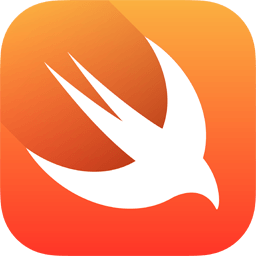
\includegraphics[width=2cm]{swift-128_2x}
\caption{Źródło: \url{https://developer.apple.com/swift/}}
\end{figure}

Objective-C było językiem w którym stworzony został framework Cocoa, pozwalający
na programowanie aplikacji na system NeXTStep, a póżniej gdy został on wykupiony 
przez apple pod koniec lat 90' XX-go wieku na platformę MacOS X. Dzięki sukcesowi
iPhone'a cieszył się on większą popularnością. I trwało to do 2014go roku gdy
został zaprezentowany język \textbf{Swift}, który zdobył serca programistów tworzących
natywny software na platformy Apple i dzisiaj już większość z nich korzysta wyłącznie
z niego.

Swift to nowoczesny język czerpiący z wielu języków najlepsze ich aspekty i 
paradygmaty. Pozwala na programowanie w pełni obiektowe, ale dzięki typom wartości
(\textit{value type semantics}) oraz przekazywanie referencji do funkcji pozwala 
również na programowanie funkcyjne. Znajdziemy w nim podobieństwa do Scali, Haskella,
Smalltalk, Clojure, Python, Ruby etc. Swift jest silnie typowanym językiem 
posiadającym klasy, których instancje przekazywane są przez referencję, struktury,
których instancje przekazywane są przez wartość, oraz protokoły, które pozwalają
na unikanie dziedziczenia poprzez stosowanie ich na klasach/strukturach. Istnieje
możliwość importowania kodu napisanego w Objective-C w Swifcie ze względu na wspólny
Runtime. Dodatkowo Swift może korzystać z kodu napisanego w C lub C++. 

Platformy, na których dostępny jest Swift to macOS, Linux oraz Windows. Jako 
projekt Open-Source jego kod źródłowy jest dostępny na portalu 
\href{https://github.com/apple/swift}{github}. W Swifcie napiszemy nie tylko
aplikację na iOS, ale również na pozostałe platformy Apple czyli macOS, watchOS
oraz tvOS\@. Isnieje również możliwość pisania serwerów, przy użyciu takich frameworków 
jak \href{https://www.kitura.io}{Kitura} czy \href{https://vapor.codes}{Vapor}.
Najnowszą wersją Swifta jest 4.2.

\subsection*{iOS SDK}
iOS dziedziczy wiele po systemie macOS\@. W skład iOS SDK (\textit{Software Development 
Kit}) wchodzą biblioteki znane już deweloperom tworzącym oprogramowanie na macOS
oraz biblioteki stworzone z myślą o urządzeniach mobilnych. CocoaTouch jest potomkiem 
frameworku Cocoa dostępnego na systemach macOS, który jest rozszerzony o interfejs 
obsługi narzędzi dostępnych w urządzeniu mobilnym takich jak rozpoznawanie gestów,
serwis lokalizacji czy obsługa kamery. W skład CocoaTouch wchodzą między innymi
biblioteki Foundation, UIKit, MapKit, EventKit i wiele innych. Dzięki temu pakietowi
Apple zdefiniowało jak powinny być tworzone aplikacje na iOS\@. Dostarczony jest 
zbiór wielu elementów interfejsu użytkownika, które można dowolnie rozszerzać i
modyfikować, aby stworzyć unikalny wygląd aplikacji trzymając się wytycznych
wyznaczonych przez Apple. Dostęp do gestów zapewni naszej aplikacji lekkość obsługi
oraz intuicyjność, a niezliczona ilość innych bibliotek wchodzących w skład
CocoaTouch sprawi, że aplikacja nabierze życia. Implementowanie funkcjonalności staje
się bardzo proste dzięki wysoko poziomowym interfejsom dającym dostęp do
poszczególnych elementów systemu oraz fizycznego urządzenia. CocoaTouch jest 
najbardziej elementarnym frameworkiem na iOS, ponieważ to on zapewnia na poziomie
podstawowym to co potrzebne do stworzenia funkcjonalnej aplikacji. 

\subsection*{AppStore}
Jedyną oficjalną drogą udostępnienia aplikacji konsumentowi jest AppStore, świetnie
znany każdemu użytkownikowi iOS\@. Aby umieścic aplikację w sklepie AppStore
należy posiadać wcześniej wspomniane konto deweloperskie Apple. Portal AppStoreConnect
pozwoli nam na zarządzanie kolejnymi wersjami aplikacji, a nawet beta-testowanie
dzięki aplikacji TestFlight. To wszystko za jedyne 99\$ rocznie. Na iOS nie istnieje
inna możliwość instalacji aplikacji niż AppStore, za wyjątkiem manulanej instalacji
przez Xcode. W tym celu najlepiej udostępniać swój kod źródłowy na githubie. Zanim 
jednak aplikacja zostanie upubliczniona w AppStore musi ona przejsc proces Review.
Apple dokładnie analizuje każdą aplikację indywidualnie, poprzez manualne testy oraz
skrypty, które mają zapewnić bezpieczeństwo oraz upewnić się, że aplikacja spełnia
wszystkie ich \href{https://developer.apple.com/design/human-interface-guidelines/ios/visual-design/adaptivity-and-layout/}{wymogi odnośnie UI oraz UX}. Proces ten może potrwać od jednego do trzech
dni, a z każdą kolejną iteracja poprawek i review okres ten będzie się przedłużał.

\begin{figure}[h]
\centering
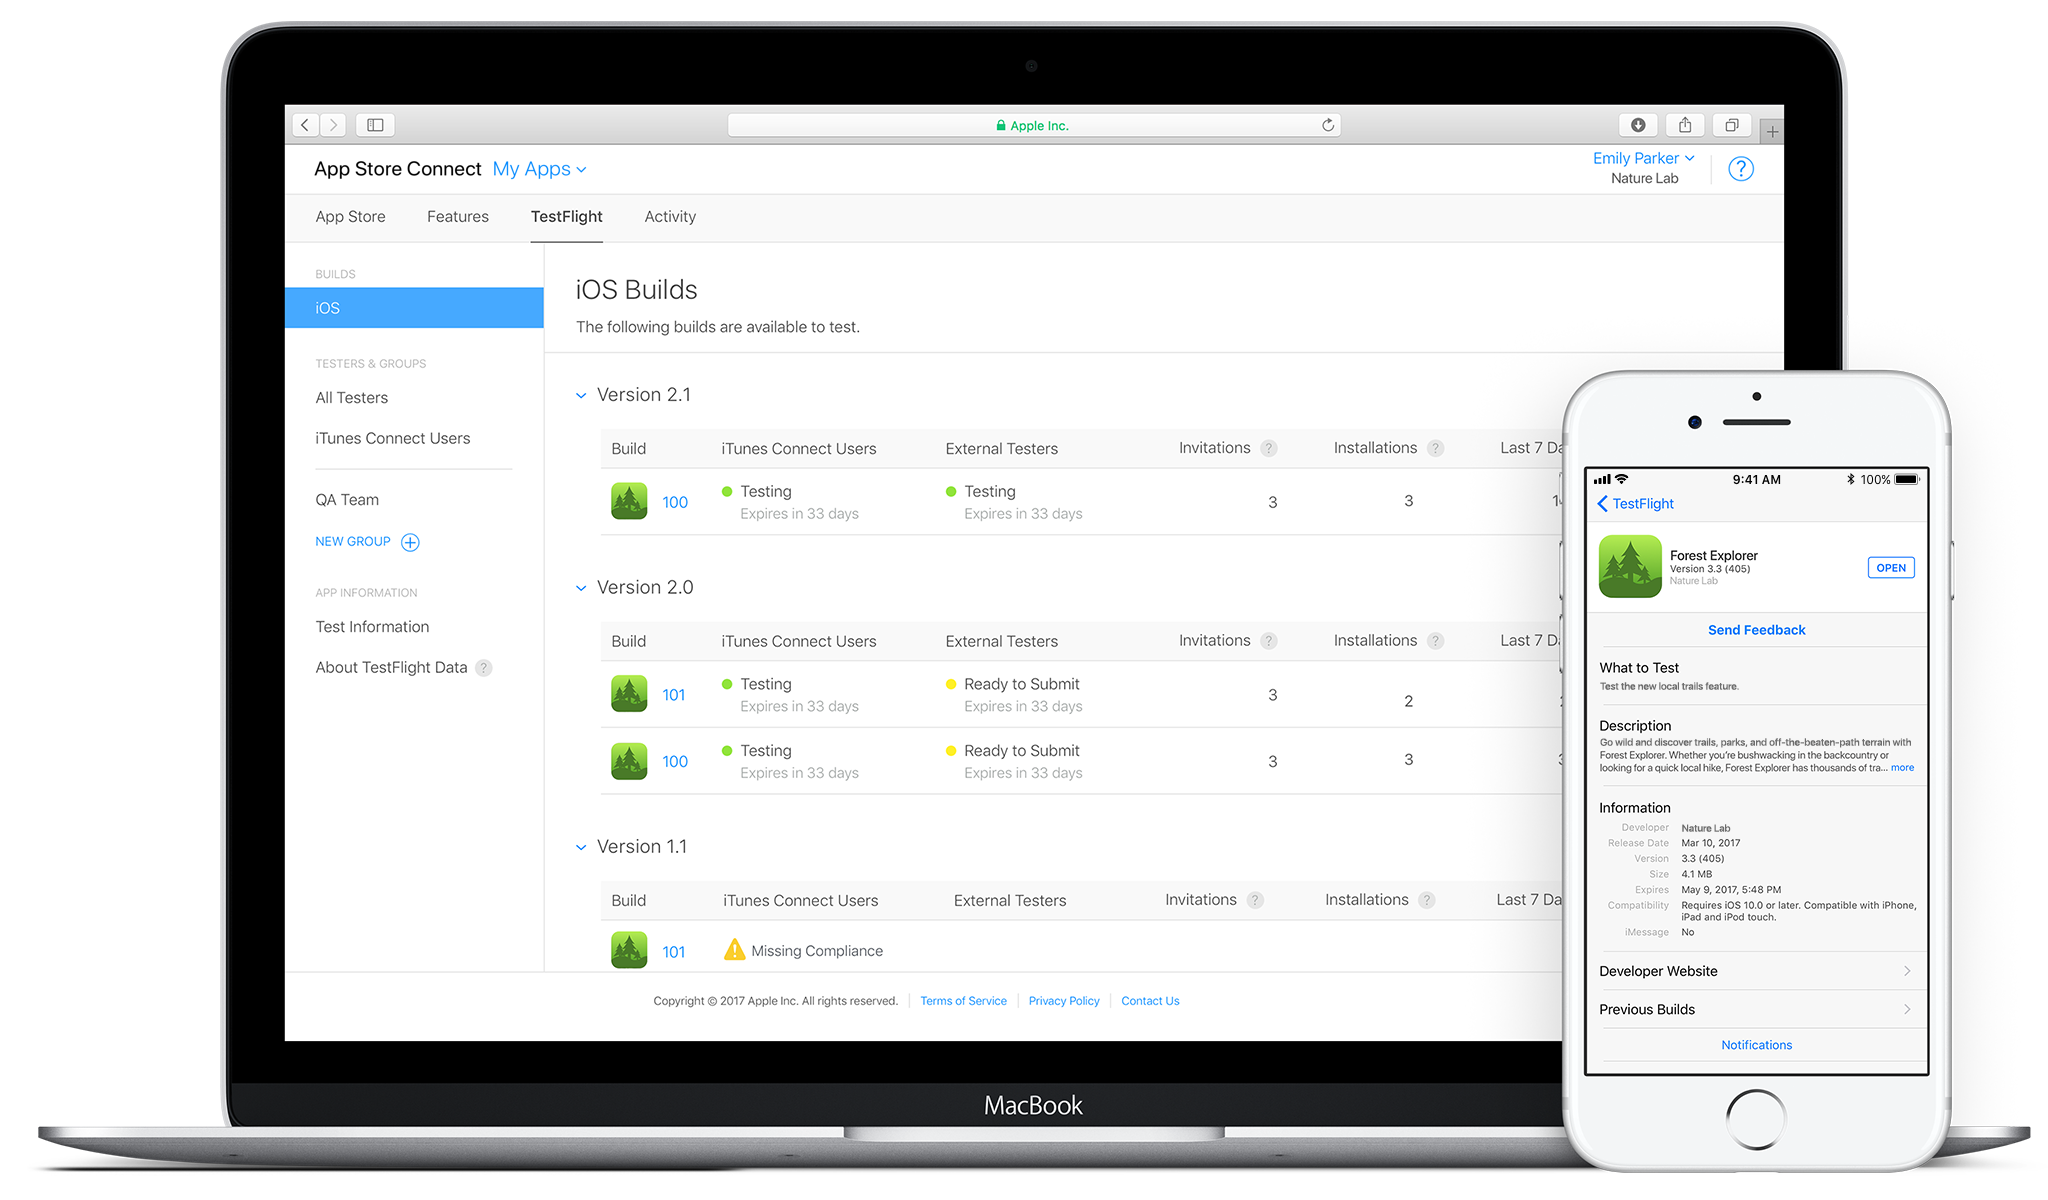
\includegraphics[width=12cm]{testflight-overview-hero-large_2x}
\caption{Źródło: \url{https://developer.apple.com/testflight/}}
\end{figure}


%
% Section: Development
%
\section*{Development}
\subsection*{Architektura}
Przedstawiłem już środowisko w jakim pracuje iOS Developer, a więc czas przejść
do części w której omówimy sam proces pisania aplikacji z punktu widzenia kodu.
Architektura, w okół ktorej zorientowane jest API dostarczane nam przez Apple
to \textbf{MVC} czyli \textit{Model-View-Controller}. I taką też stosuje się w 
większości aplikacji. Platforma istnieje na tyle długo, że zaczeły powstawać różne
wariancje MVC np. MVVM \textit{Model-View-ViewModel}, oraz zaczęto stosować 
architektury znane z innych platform takie jak \textit{The Elm Architecture} i 
\textit{Clean Architecture}, lub inna jego interpretacja \textit{Viper}. Każdy 
doświadczony deweloper bedzie miał swoją opinię dotyczącą każdej z nich, lecz
nad jednym będą zgadzać się wszyscy --- najważniejsze w czym powstanie dana aplikacja,
lecz ważne to aby podejscie było spójne i czyste na przestrzeni całego kodu.
MVC nie cieszy się najlepszą reputacją, ze względu na to, że łatwo można przesadzić
z ilościa zadań i odpowiedzialności danego komponentu. Co jest defacto błędem
programisty aniżeli sammego patternu.

Jeżli chodzi o wzorce projektowe, to najpowszechniejszym z pewnością będzie 
\textbf{Delegate Pattern}. Jest on wykożystywany masowo w iOS SDK, wiec i naturalnie
jest on adaptowany przez programistów w aplikacjach. Pewną alternatywą będzie tutaj 
stosowanie reaktywnego programowania. Do tego zazwyczaj korzysta się z trzecich
bibliotek takich jak \textbf{RxSwift/RxCocoa} lub \textbf{ReactiveSwift/ReactiveCocoa}.
Biblioteki te opierają się przedewszystkim na \textbf{Observer Pattern}. Podczas 
gdy w typowej aplikacji napisanej w MVC najczęściej spotkamy wzorzec Delegata,
to w tych napisanych przy użyciu MVVM reaktywne biblioteki zazwyczaj będą szły 
z nim w parze. A skoro mowa o wzorcu MVVM to warto wspomnieć o pewnej jego wersji,
MVVM+C --- \textit{MVVM+Coordinators}. Coordynatory w tym przypadku odpowiedzialne
będą za nawigację miedzy poszczegółnymi ekranami i scenariuszami. Nieżadko spotkamy 
równierz takie wzorce jak \textbf{Dependency Injection}, \textbf{Factory Pattern}
oraz \textbf{Builder Pattern}. W aplikacji demonstracyjnej dołączonej do tego artykułu
został wykożystany MVC w swojej najczystszej formie.

\subsection*{UIKit}
\textbf{UIKit} Jest frameworkiem, który dostarcza nam podstawowe klasy widoków oraz
kontrollerów, a są nimi \textbf{UIView} oraz \textbf{UIViewController}. W celu 
stworzenia własnego widoku lub kontrolera należy subclassować odpowiednią podstawową
klasę aby UIKit mógł opowiednio wyświetlić oraz zarządzać danym widokiem. W UIKit
znajdziemy dodatkowo całą masę widoków i kontrolek, które są wykorzystywane w
aplikacjach systemowych. Dobrą praktyką jest wykorzystywanie tych klas w celu
utrzymania jednolitego wyglądu platformy oraz aby zapewnić użytkownikowi najlepszy 
experience. Uzytkownik będzie wiedział dzięki temu jakiej reakcji ma się spodziewać
gdy dokona jakiejś czynności. Właśnie to powoduje, że iOS jest tab bardzo przystępny
zwykłemu userowi. Ujednolicony design oraz flow aplikacji sprawia, że osobie która
po raz pierwszy trzyma w ręku iPhone bądź inne urządzenie z iOS, bardzo szybko
się oswaja z gestami i zachowaniami systemu.

\begin{figure}[h]
\centering
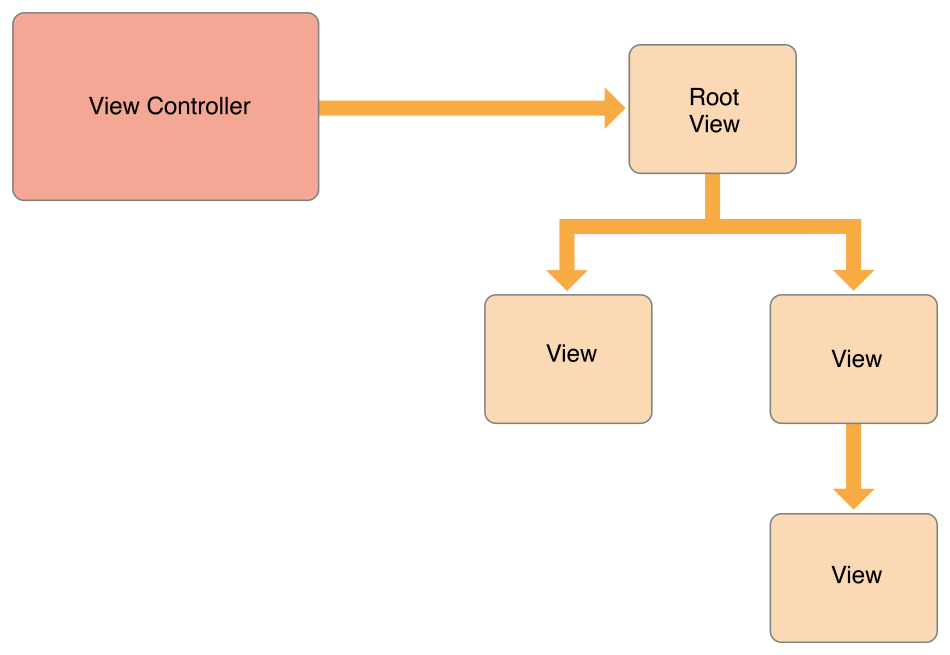
\includegraphics[width=8cm]{viewcontroller-relationship}
\caption{Relacja między UIViewController a instancjami UIView}
\end{figure}

Aplikacja demonstracyjna składa się z czterech ekranów, a za każdy z nich odpowiada
jedna klasa dziedzicząca po UIViewController. Są to:
\begin{enumerate}
    \item{CategoriesViewController}
    \item{ProductsViewController}
    \item{ProductDetailsViewController}
    \item{MapViewController}
\end{enumerate}
Zachęcam do przeanalizowania indywidualnie do kodu każdego z tych kontrollerów.
To na co należy zwrócic uwagę to przedewszystkim metoda \textit{viewDidLoad}.
UIKit woła tą metodę, gdy widok zostanie poprawnie załądowany z pliku XIB bądż
Storyboard (o czym wktórce) i to tutaj powienien się wykonać kod konfigurujący 
widoki danymi z modelu.

\subsection*{Storyboardy}
Podczas omawiania Xcode wspomniałem o pewnej jego funkcjanalności, a konkretnie 
o Interface Builder. Teraz jest opowiedni moment aby ten temat rozwinąć, ponieważ
mowiąc o tworzeniu aplikacji na iOS nie można ominąć tematu Storyboardów. Pliki
Storyboard zawierają informacje o tym jak wygląda nasza aplikacja, jak poszczególne
widoki się na siebie nakładają, w jaki sposób są ułożone oraz kolejnośc w jakiej 
zostają pokazywane. Są one edytowalne na dwa sposoby, z czego pierwszy z nich nie
ma kompletnie sensu ponieważ tak naprawdę mamy tutaj do czynienia z zazwyczaj gigantycznym
plikiem XML, który nie wiele nam mowi. Głównym i jedynym rozsądnym sposobem edycji jest
wbudowany w Xcode Interface Builder. Pozwala on nam na układanie widoków jak `klocki'
w dość trywialny sposób.

\begin{figure}[h]
\centering
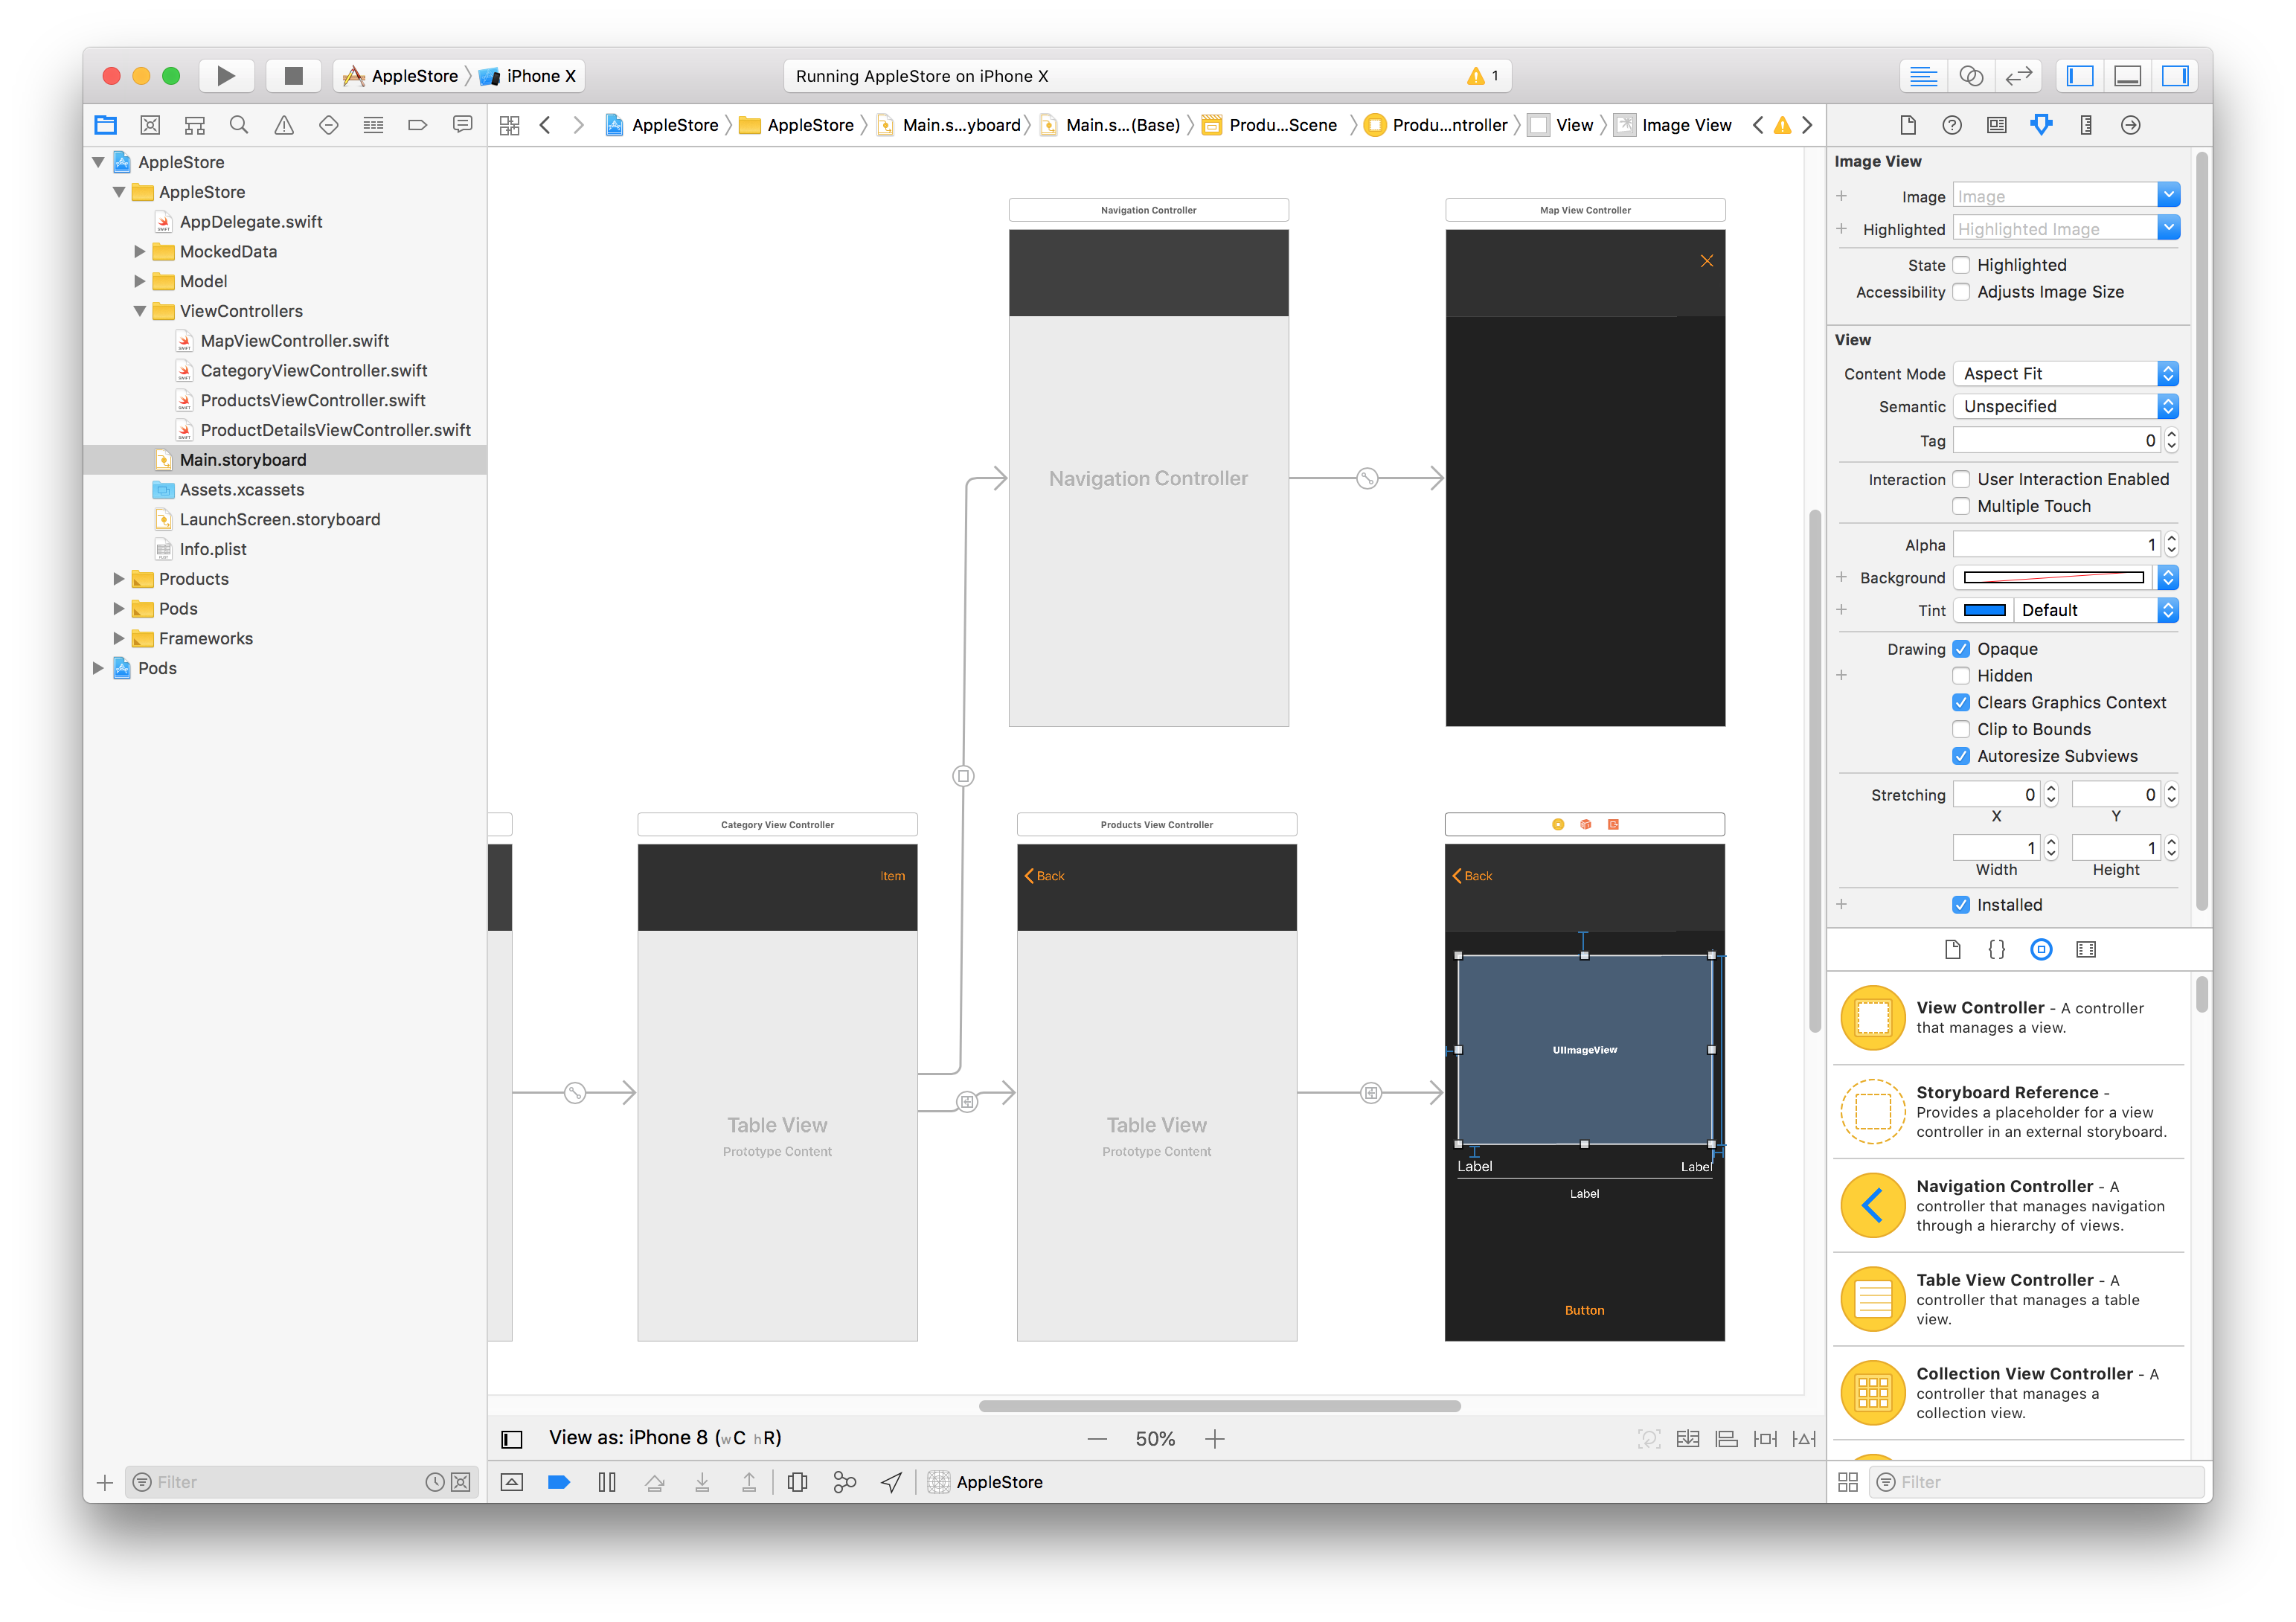
\includegraphics[width=12cm]{xcode-interfacebuilder}
\caption{Plik Main.storyboard w Inteface Builder (Xcode)}
\end{figure}

\subsection*{Zarządzanie Paczkami}
Każda techonologia posiada jakieś menadżery zależności. W świecie Swifta są trzy
najpopularniejsze managery. Konkurs popularności z pewnością zwyciężyły by 
\textbf{CocoaPods} --- Zcentralizowany \textit{Package Manager}, który w bardzo 
prosty dołączyc dependencje do projektu Xcode-owego. Ingeruje on dość mocno w 
plik projektu i z pewnością nie jest on idealny. Alternatywą dla niego będzie
\textbf{Carthage}. Ten natomiast odpowiedzialny będzie głównie za budowanie dependencji,
a podpinanie ich pod projekt pozostawia programiście. Jego zaletą jest brak 
ingerencji w projekt oraz fakt iż jest to zdecentralizowany menadżer. Wystarczy
wskazać mu repozytorium githubowe a zaciągnie on jego zawartość oraz zbuduje
na wskazaną platformę. Ostatnią opcją będzie \textbf{Swift Package Manager}. Jest 
on jeszcze w dość wczesnej fazie rozwoju i aktualnie nie wspiera iOS, jednakże
można wykorzystać go w projektach, które stworzone są na takie platformy jak linux
(Server-side Swift). SPM z pewnościa doczeka się wsparcia dla iOS, lecz może to 
potrwac nawet do kilku lat. Kazdy z wymienionych przeze mnie Package Managerów 
jest open sourcowym projektem któego pliki źródłowe można zobaczyć na githubie.

\subsection*{Symulator}
\textbf{Simulator} robi dokładnie to czego można się po nim spodziewać. Pozwala
nam na uruchomienie aplikacji na symulatorze dowolnego urządzenia z systemem iOS\@.
Alternatywą jest oczywiście budowanie i instalacja aplikacji na urządzeniu fizycznym 
podłączonym poprzez kabel USB lub bezprzewodowo przez WiFi. Należy jednak pamiętać,
że aplikacje udostępnia się na wiele urządzeń, z różnymi rozmiarami ekranów. 
Dzięki symulatorowi przetestujemy nasza aplikację na każdym z wspieranych najnowszym
system urządzeń. Jedynym minusem jest oczywiście fakt, że nie użyjemy na nim aplikacji
w ten sam sposób w jaki zrobilibyśmy to na fizycznym urządzeniu. Z pewnością będzie
jednak on nam przydany podczas budowania interfejsów.

\begin{figure}[h]
\centering
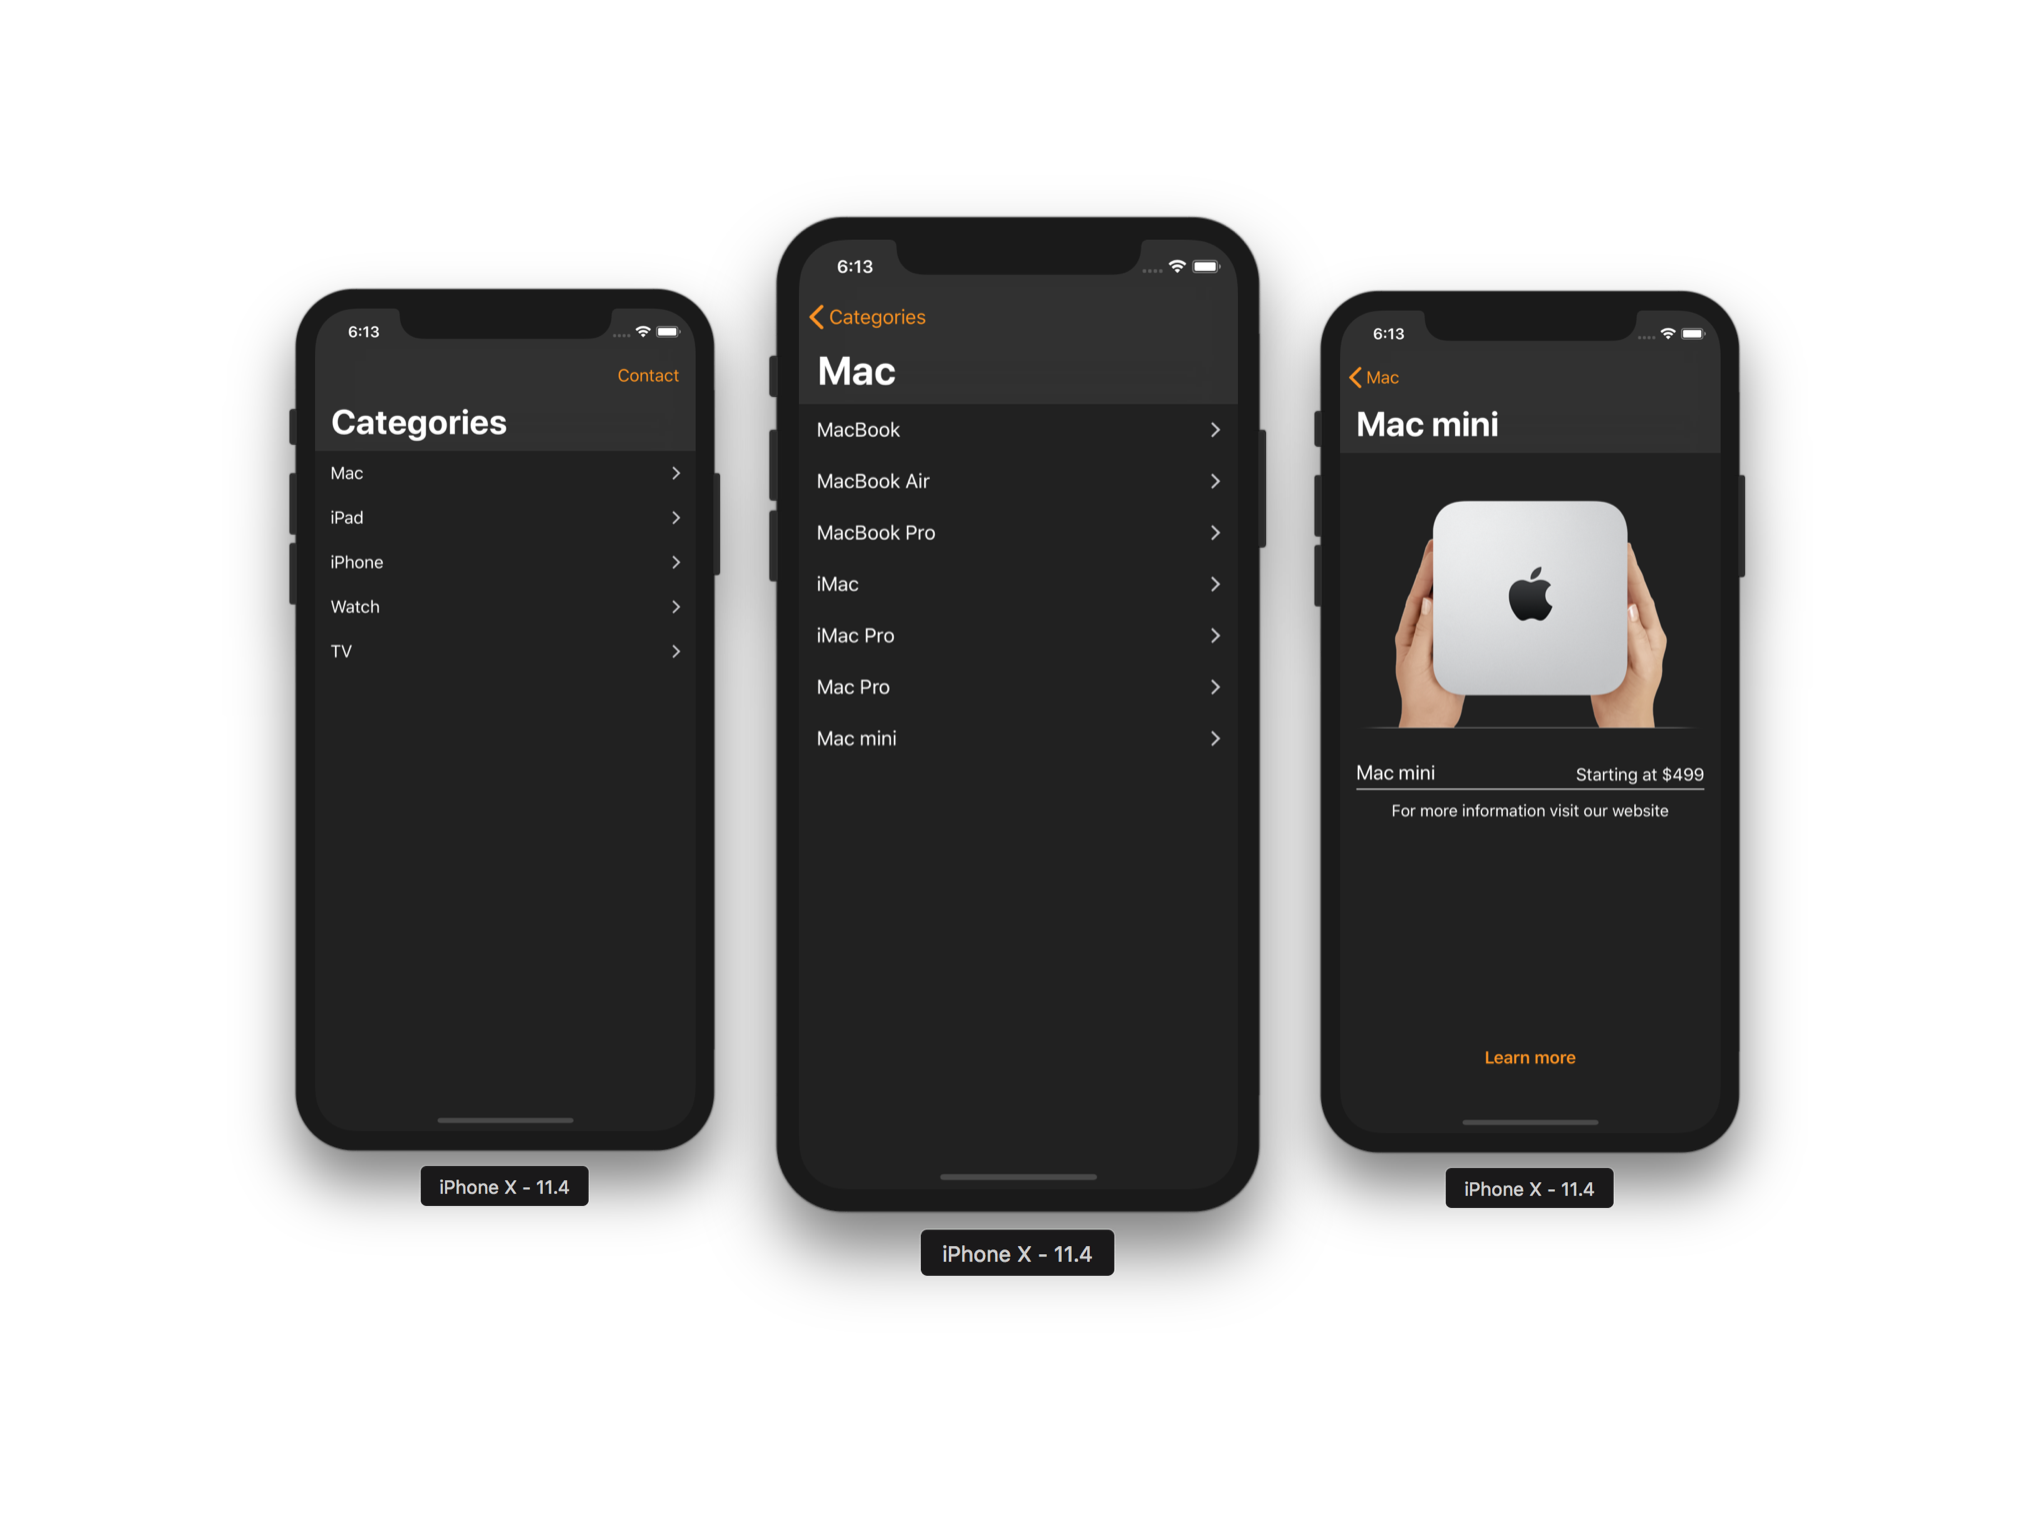
\includegraphics[width=12cm]{apple-store-app-screens}
\caption{Aplikacja demonstracyjna uruchomiona w symulatorze iPhone X}
\end{figure}

\section*{Podsumowanie}
Czy tworzenie aplikacji jest dla Ciebie? Jest to pytanie, na które tylko ty możesz
sobie odpowiedzieć. Jeżeli pasjonuje cię tworzenie płynnych interfejsów i łączenie
ich z najnowszymi nowinkami technicznymi, którymi przepchanę za w dzisiejszych czasach
komputery, które nosimy w naszych kieszeniach. Zbudowanie prostej aplikacji jest
raczej nie trudnym zadaniem, a przynosi ogromną satysfakcję gdy widzi się efekty.
A najlepszym aspektem tego może być fakt że twoja aplikacja może trafić do setek 
tysięcy telefonów na całym świecie. System iOS z pewnością nie zniknie z rynku, 
a przynajmniej nie w tej dekadzie. Apple osiąga rekordowe wyniki sprzedaży oraz
spory procent udziału na rynku smartfonów należy do iPhone. Zrewolucjonizował on
to czym jest telefon, ale przedewszystkim to w jaki sposób pracujemy na codzień.
Dla programisty oznacza to ogromne pole to popisu. Jeżeli chcesz wziąć udział w
tej rewolucji możesz zaczać tworzyć aplikacje już teraz i wpływać na życie ludzi.

\end{document}
